
\documentclass[a4paper,10pt]{article}
\usepackage{graphicx}
\usepackage{caption}
\usepackage{subcaption}
\usepackage{amsmath}
%opening
\title{Report Exercise 4}
\author{Marion Baumgartner}

\begin{document}

\maketitle

\section{Task 1: Calculate the average distance between particles}

\begin{figure}[h]
\centering
 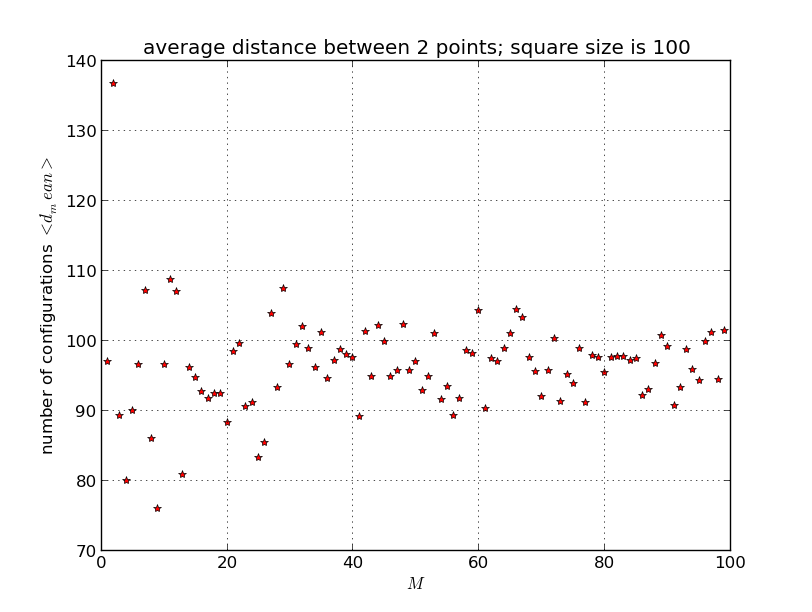
\includegraphics[width=0.4\textwidth]{sol2}
 \caption{}
\label{fig1}
\end{figure}

\begin{figure}[h]
\centering
 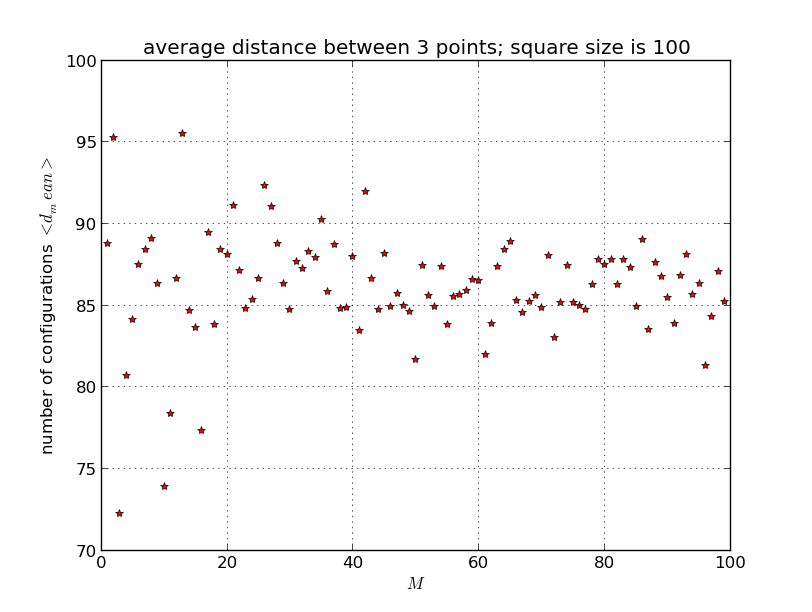
\includegraphics[width=0.4\textwidth]{sol3}
 \caption{}
\label{fig2}
\end{figure}

\begin{figure}[h]
\centering
 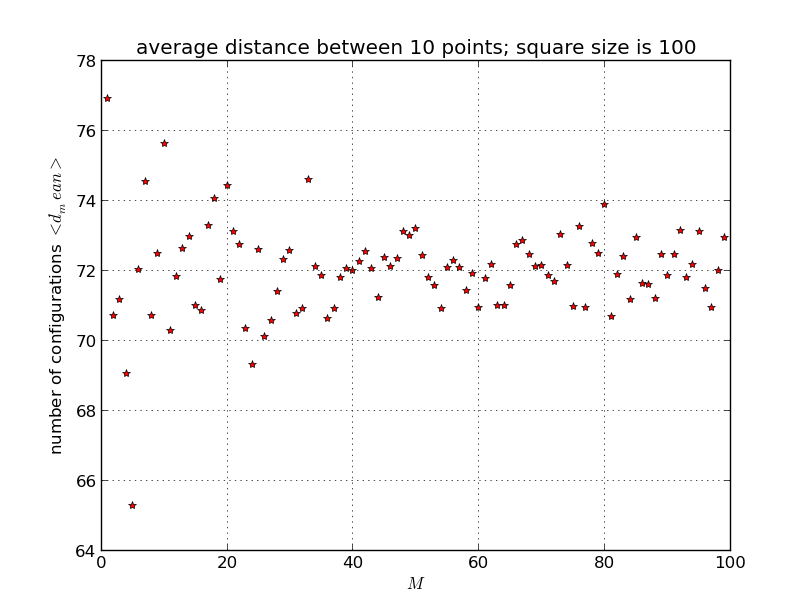
\includegraphics[width=0.4\textwidth]{sol10}
 \caption{}
\label{fig3}
\end{figure}

\begin{figure}[h]
\centering
 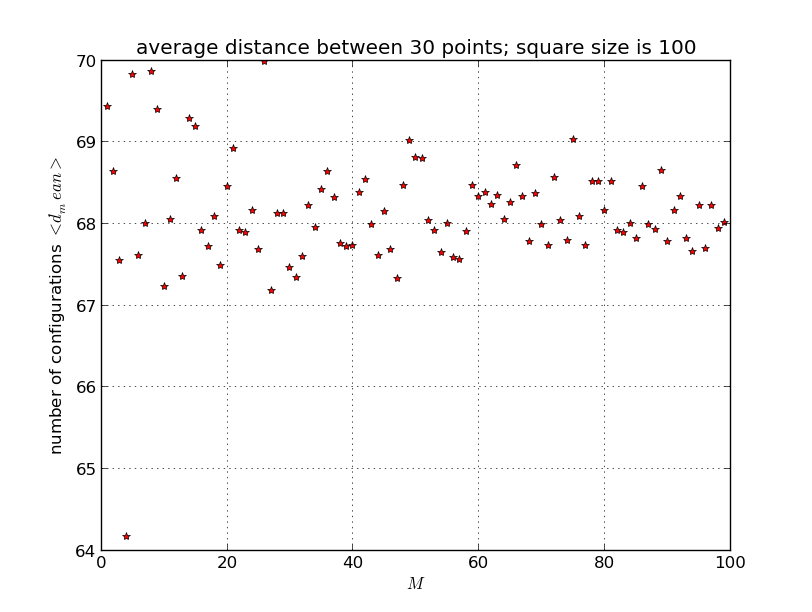
\includegraphics[width=0.4\textwidth]{sol30}
 \caption{}
\label{fig4}
\end{figure}


\begin{figure}[h]
\centering
 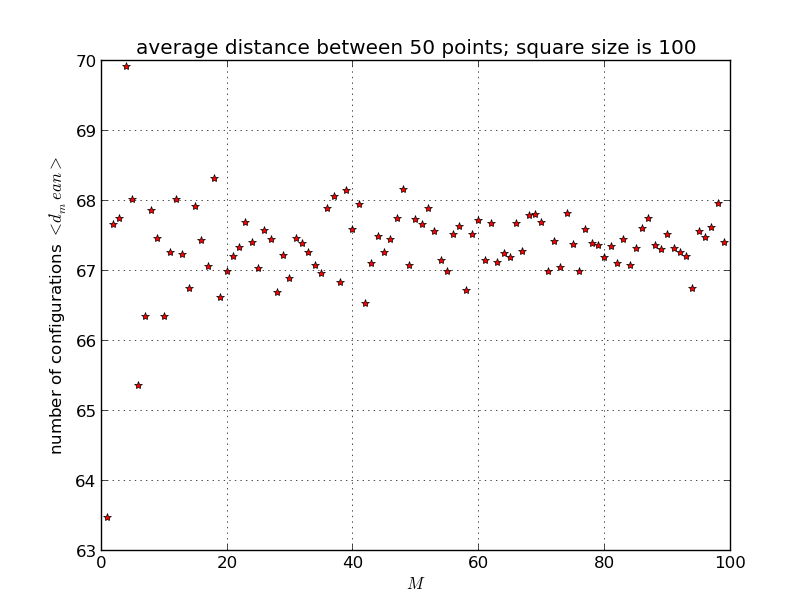
\includegraphics[width=0.4\textwidth]{sol50}
 \caption{}
\label{fig5}
\end{figure}

The figures \ref{fig1} to \ref{fig2} show the average distance petween particles in a box of lenth $L=100$. All the particle spheres have a radius $R=0.05$. $L$ and $R$ is kept the same for all the images named above, in order to be able to compare them. In these images i used diffren amount of spheres $n$ in the box, the number is given above each figure.

What we can see in these figures is that with an increasing numeber of shperes in the box the plot shows a more stable figure. For the plots with low $n$ we have a large scatter for small $M$. This improves if we increas the number. Looking at figure \ref{fig5}, for $M\in \[60,100\]$ the scatter is within a range of $<d_{mean}\in \[67,68\]$ . In comparison with figure \ref{fig1}. Here we have a range of  $<d_{mean}\in \[90,110\]$ whi is a range $20$ times larger than for figure \ref{fig5}.

If we compare figure \ref{fig5} with figures \ref{fig3} and \ref{fig4} it can be observed that we get less scatter for smaller M in figure \ref{fig5}.

In the figures \ref{} to ref{} I kept $n$ the same and varied the radius of the spheres $R=1,5,10$




\begin{figure}
        \centering
        \begin{subfigure}[b]{0.3\textwidth}
		\centering
		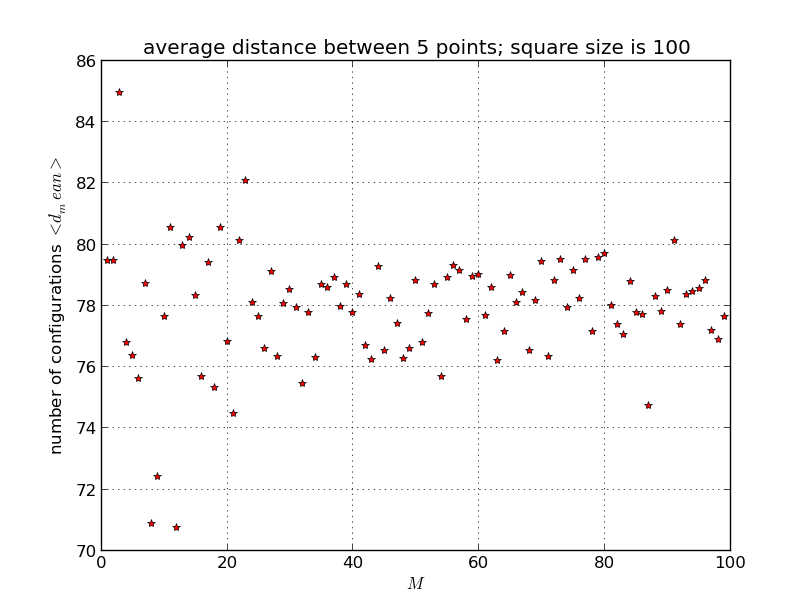
\includegraphics[width=0.4\textwidth]{solR1n5}
        \end{subfigure}%
        ~ %add desired spacing between images, e. g. ~, \quad, \qquad etc. 
          %(or a blank line to force the subfigure onto a new line)
        \begin{subfigure}[b]{0.3\textwidth}
		\centering
		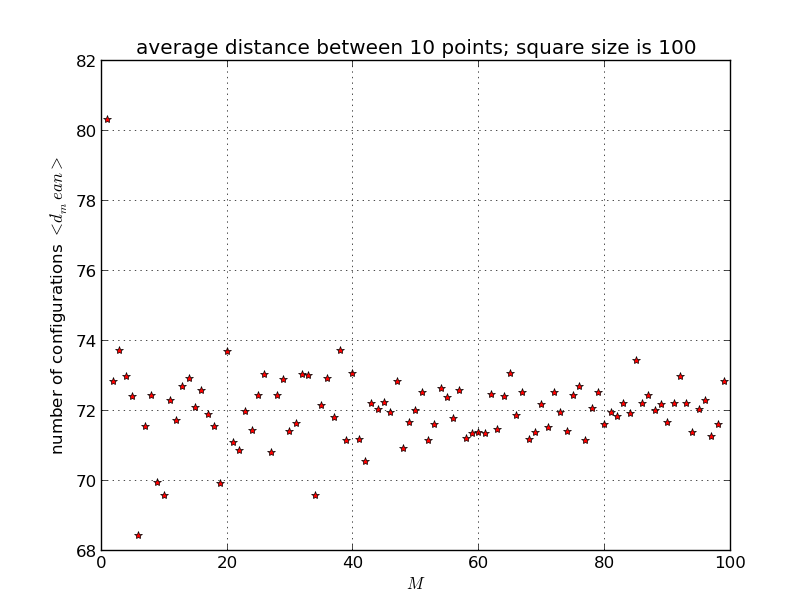
\includegraphics[width=0.4\textwidth]{solR1n10}
        \end{subfigure}%
        ~ %add desired spacing between images, e. g. ~, \quad, \qquad etc. 
          %(or a blank line to force the subfigure onto a new line)
        \begin{subfigure}[b]{0.3\textwidth}
		\centering
		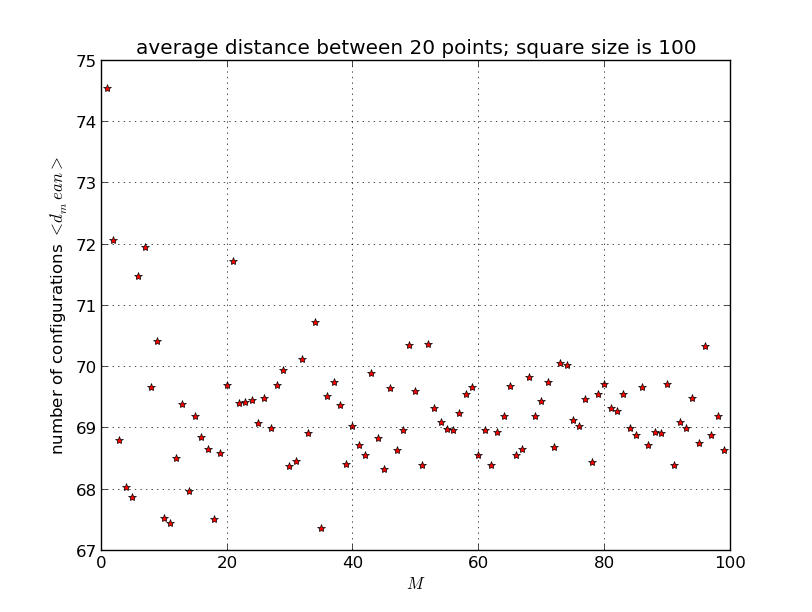
\includegraphics[width=0.4\textwidth]{solR1n20}
        \end{subfigure}
        ~ %add desired spacing between images, e. g. ~, \quad, \qquad etc. 
          %(or a blank line to force the subfigure onto a new line)
        \begin{subfigure}[b]{0.3\textwidth}
		\centering
		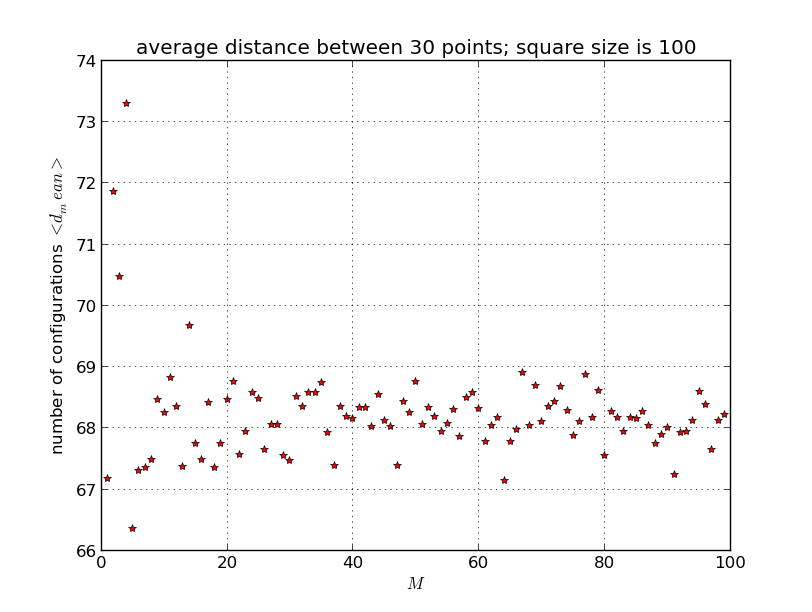
\includegraphics[width=0.4\textwidth]{solR1n30}
		\caption{}
		\label{fig5}
        \end{subfigure}
        \caption{Pictures of animals}
        \label{fig:animals}
\end{figure}

\begin{figure}
        \centering
        \begin{subfigure}[b]{0.3\textwidth}
		\centering
		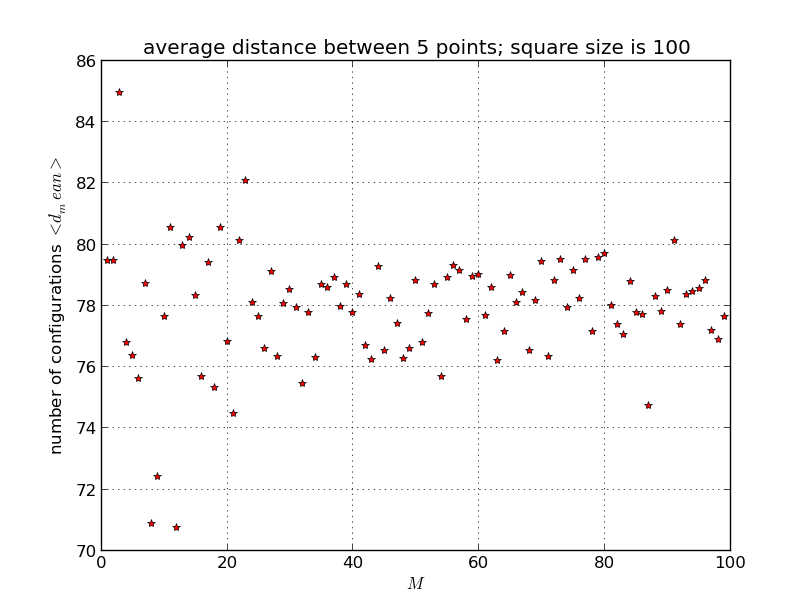
\includegraphics[width=0.4\textwidth]{solR1n5}
        \end{subfigure}%
        ~ %add desired spacing between images, e. g. ~, \quad, \qquad etc. 
          %(or a blank line to force the subfigure onto a new line)
        \begin{subfigure}[b]{0.3\textwidth}
		\centering
		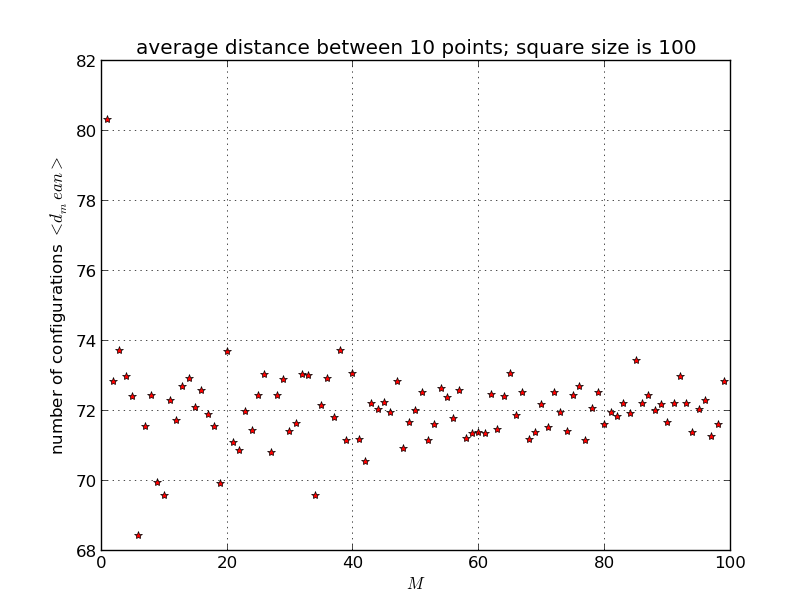
\includegraphics[width=0.4\textwidth]{solR1n10}
        \end{subfigure}%
        \caption{Pictures of animals}
        \label{fig:animals}
\end{figure}

\begin{figure}
        \centering
        \begin{subfigure}[b]{0.3\textwidth}
		\centering
		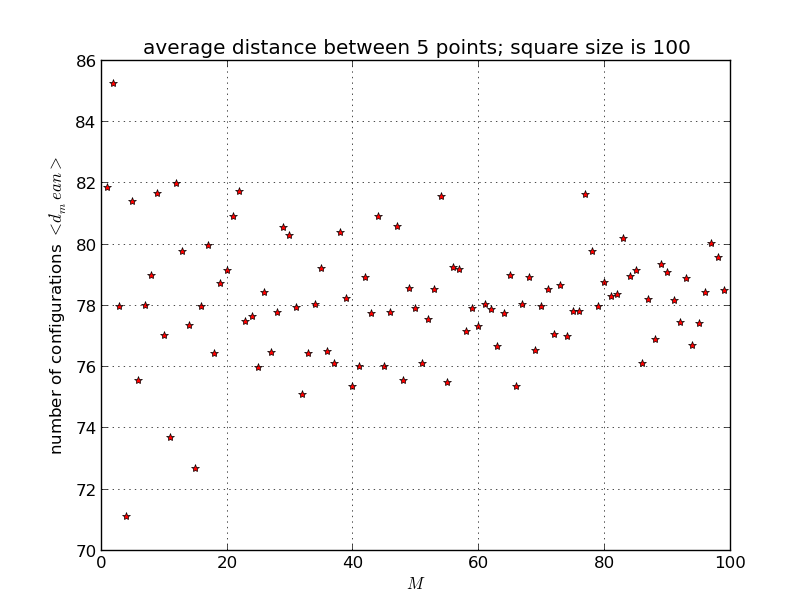
\includegraphics[width=0.4\textwidth]{solR5n5}
        \end{subfigure}%
        ~ %add desired spacing between images, e. g. ~, \quad, \qquad etc. 
          %(or a blank line to force the subfigure onto a new line)
        \begin{subfigure}[b]{0.3\textwidth}
		\centering
		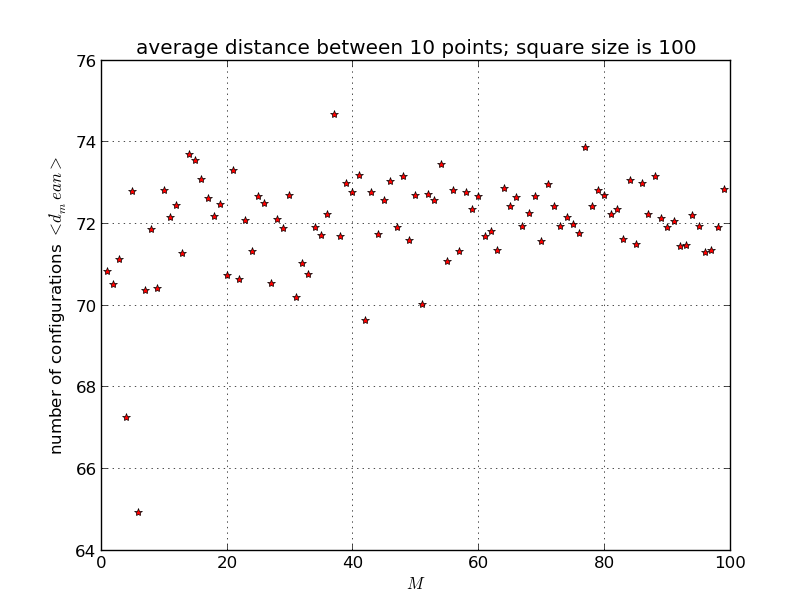
\includegraphics[width=0.4\textwidth]{solR10n10}
        \end{subfigure}%
        \caption{Pictures of animals}
        \label{fig:animals}
\end{figure}


In the table \ref{bla} I calculated the total sphere volume and the volume fraction $\nu$ for all the different combinations of $n,R$ and $L$ which I used to generate the figures.


\begin{table}
  \begin{tabular}{|c|c|c|c|c|c|}
  \hline
   $L$& $R$&$n$&$\nu$&$\gamma$ \\ \hline
   \multirow{3}{*}{100} & \multirow{3}{*}{0.05} &$n$&$\nu$&$\gamma$ \\ \hline
  
  \end{tabular}
  \caption{ sphere volume and the volume fraction $\nu$ for all the different combinations of $n,R$ and $L$ which are used to generate the figures.}
  \label{tabel1}
\end{table}

\end{document}
